\section{Implementation}


In section~\ref{sec:dataset} we describe the data set that we use, 
then we describe how we extract identifiers from this dataset 
(section~\ref{sec:defextraction-impl}) and how this dataset is cleaned
(section~\ref{sec:datacleaning}). Next, the implementation of clustering
algorithms is described in the section~\ref{sec:datacleaning}. After
the clusters are found, we combine them into a hierarchy in 
the section~\ref{sec:hierarchy}. 

Finally, in the section~\ref{sec:jlp} we explore how the same set of techniques
can be applied to source code in Java.


\subsection{Data set} \label{sec:dataset}

In this work we apply the discussed techniques to the English version of
Wikipedia \cite{enwikidump}.
It's a big web encyclopedia where articles are written and edited by 
the community. For our work wikipedia is interesting because 
there are many math pages. 


At present (\today) English wikipedia contains about 4.9 mln
articles\footnote{\url{https://en.wikipedia.org/wiki/Wikipedia:Statistics}}
and it is 1.5 Gb in the compressed form. However, only a small portion
of these articles are math related: only about 30.000 pages contain at least 
one \verb|<math>| tag. 

The math information is enriched with semantic information by MediaWiki 
and we use this augmented data representation. 30.000 math pages with 
augmented math tags occupy around 1.5 Gb in uncompressed form. 

Apart from the text data and formulas wikipedia articles have information
about categories, which can also be exploited. It is hard to 
extract category information from the raw wikipedia mark up, but this 
information is available in a structured form in DBPedia \cite{bizer2009dbpedia}.


\subsection{Definition Extraction} \label{sec:defextraction-impl}

Before we can proceed to discovering identifier namespaces, we  
need to extract identifier-definition relations. For this we use the probabilistic 
approach, discussed in the section~\ref{sec:mlp}. 
The extraction process in implemented using Apache Flink \cite{flink}.

But before the original dataset can be preprocessed, it is enriched with 
augmented MathML (see section~\ref{sec:mathml}), 
and then the dataset is filtered such that only articles with
the math tag are retained. 

In the wikipedia dataset each document is represented using wiki XML. It 
makes it easy to extract title and content, and then, the all the formulas 
are extracted from the content. The formulas are extracted by 
looking for \verb|<math>| tags. However some formulas are typed without 
the tag, but only with unicode characters. Such formulas are not easy to 
detect and therefore in this word we choose not to process them.
Once all \verb|<math>| tags are found, they (along with the content) 
are replaced with a special placeholder \verb|FORMULA_%HASH%|, where 
\verb|%HASH%| is MD5 hash \cite{rivest1992md5} of the tag's content represented as 
a hexadecimal string. After that 
the content of the tags is kept separately from the document content. 

Once formulas are retrieved, we extract the definitions from them. 
We are not interested in the semantics of a formula, only in the identifiers 
it contains. Hence we need only to look for all \verb|<ci>| tags. 
There are two types of identifiers: simple identifiers such as 
``$t$'', ``$C$'', ``$\mu$''; and complex identifiers with subscripts such as
``$x_1$'', ``$\xi_i$'' or even ``$\beta_{\text{slope}}$''. We do not process 
superscripts because they are usually powers (for example, $x^2$), 
and therefore they are not interesting for this work. 
There are exceptions to this, for example, ``$\sigma^2$'' is an identifier,
but these cases are rare and can be ignored. 

Since MathML is XML, the identifiers are extracted with XPath queries:

\begin{itemize}
  \item \verb|//m:mi[not(ancestor::m:msub)]/text()| for all \verb|<ci>| tags
that are not subscript identifers
  \item \verb|//m:msub| for subscript identifiers
\end{itemize}

Once the identifiers are extracted, the rest of the formula is discarded. 
As the result, we have a ``Bag of Formulas''.

The content of a wiki document is structured and authored with a special 
markup language for specifying document layout elements such as
headers, lists, text formatting and tables: Wiki markup. 
Thus the next step is to process the Wiki markup and extract the textual 
content of an article, and this is done using a Java library 
``Mylyn Wikitext'' \cite{mylynwikitext}.
Almost all annotations are discarded at this stage,
and only inner-wiki links are kept: they can be useful as candidate definitions.

Once the markup annotations are removed and the text content of an article is 
extracted, we then apply Natural Language Processing (NLP) techniques.
Thus, the next step is the NLP step, and for NLP we use StanfordNLP
\cite{manning2014stanford}. 
The first part at this stage is to tokenize the text and also split it by sentences. 
Once it is done, we then apply Math-aware POS tagging
(see section~\ref{sec:postagging}).
For identifiers and math formulas we introduce two new POS classes: 
``\verb|ID|'' and ``\verb|MATH|'', respectively. 
These classes are not a part of the 
standard Penn Treebank POS Scheme \cite{santorini1990part} used by 
StanfordNLP, therefore we need to label all the instances of these tags ourselves 
during the additional post-processing step. If a token starts
with ``\verb|FORMULA_|'', then we recognize that it is a placeholder 
for a math formula, and therefore we annotate it with the ``\verb|MATH|''
tag. Additionally, if this formula contains only one identifier, this 
placeholder token is replaced by the identifier and it is tagged with 
``\verb|ID|''. Additionally, we keep track of all identifiers found in 
the document and then for each token we check if this token is in the list. 
If it is, then it is re-annotated with ``\verb|ID|'' as well.

At the Wikipedia markup processing step we discard almost all markup 
annotations, but keep only inter-wiki links, because these links
are good definition candidates. To use them, we introduce 
another POS Tag: ``\verb|LINK|''. To detect all inner-wiki links, 
we first find all token subsequences that start with \verb|[[| 
and end with \verb|]]|. 
Then these subsequences are concatenated and tagged as ``\verb|LINK|''.

Also we are interested in all sequences of successive nouns (both singular 
and plural) possibly modified by an adjective. We concatenate all
such sequences into one token tagged with ``\verb|NOUN_PHRASE|''.


Next we select the most probably identifier-definition pairs. 
At this stage we are interested only in tokens annotated with  ``\verb|LINK|''
and ``\verb|NOUN_PHRASE|'': these tokens are definition candidates, and 
we rank each token by a score that depends how far it is from the identifer
of interest and how far is the closest formula that contains this 
identifier (see section~\ref{sec:mlp}). 
The output of this step is a list of identifier-definition pairs along 
with the score. Only pairs with scores above the user specified  
threshold are retained. 

The following is the list of the most common identifier-definition pairs:

\begin{itemize}
\item $t$: ``time'' (1086)
\item $m$: ``mass'' (424)
\item $\theta$: ``angle'' (421)
\item $T$: ``temperature'' (400)
\item $r$: ``radius'' (395)
\item $v$: ``velocity'' (292)
\item $\rho$: ``density'' (290)
\item $G$: ``group'' (287)
\item $V$: ``volume'' (284)
\item $\lambda$: ``wavelength'' (263)
\item $R$: ``radius'' (257)
\item $n$: ``degree'' (233)
\item $r$: ``distance'' (220)
\item $c$: ``speed of light'' (219)
\item $L$: ``length'' (216)
\item $n$: ``length'' (189)
\item $n$: ``order'' (188)
\item $n$: ``dimension'' (185)
\item $n$: ``size'' (178)
\item $M$: ``mass'' (171)
\end{itemize}



\subsection{Data Cleaning} \label{sec:datacleaning}

The Natural Language data is famous for being noisy and hard to 
clean \cite{sonntag2004assessing}. The same is true for 
mathematical identifiers and  scientific texts with formulas. 
In this section we describe how the data was preprocessed and 
cleaned at different stages of Definition Extraction 
(section~\ref{sec:defextraction-impl}).


Often identifiers contain additional semantic information visually conveyed 
by special diacritical marks or font features. For example, the diacritics can be   
hats to denote ``estimates'' (e.g. ``$\hat w$''), bars to denote the expected value 
(e.g. ``$\bar X$''), arrows to denote vectors (e.g. ``$\overrightarrow x$'') and others.
As for the font features, boldness is often used to
denote vectors (e.g. ``$\mathbf w$'') or matrices (e.g. ``$\mathbf X$''), calligraphic fonts are 
used for sets (e.g. ``$\mathcal H$''), double-struck fonts often denote spaces 
(e.g. ``$\mathbb R$''), etc. 
Unfortunately there is no common notation established across all fields of
mathematics and there is a lot of variance. For example, 
a vector can be denoted by ``$\overrightarrow x$'', ``$\boldsymbol x$'' or ``$\mathbf x$'', 
and a real line by ``$\mathbb R$'', ``$\mathbf R$'' or ``$\mathfrak R$''. 
Therefore we discard all this additional information, such that
``$\bar X$'' becomes ``$X$'', ``$\mathbf w$'' becomes ``$w$'' and ``$\mathfrak R$'' 
becomes ``$R$''.


The diacritic marks can easily be discarded because they are represented 
by special MathML instructions that easily can be ignored 
(see the section~\ref{sec:mathml} for details). But, on the other hand,
the visual features are encoded directly on the character level: 
the identifiers use special unicode symbols to convey font features such 
as boldness or Fraktur, so it needs to be normalized by converting characters
from special ``Mathematical Alphanumeric Symbols'' unicode block \cite{allen2007unicode}
back to the standard ASCII positions (``Basic Latin'' block).

Additionally, the is a lot of noise on the annotation level in MathML formulas: 
many non-identifiers are captures as identifiers inside \verb|<ci>| tags. Among 
them there are many mathematic-related symbols
like ``\textasciicircum'', ``\#'',``$\forall$'', ``$\int$''; 
miscellaneous symbols like ``$\diamond$'' or
``$\circ$'', arrows like ``$\to$'' and ``$\Rightarrow$'', and special characters like
``$\lceil$''.

To filter out these one-symbol false identifiers we fully exclude all characters from 
the following unicode blocks: ``Spacing Modifier Letters'', ``Miscellaneous Symbols'', 
``Geometric Shapes'', ``Arrows'', ``Miscellaneous Technical'', ``Box Drawing'', 
``Mathematical Operators'' (except ``$\nabla$'' which is sometimes used as an identifier)
and ``Supplemental Mathematical Operators'' \cite{allen2007unicode}.
Some symbols (like ``='', ``+'', ``\verb|~|'', ``\%'', ``?'', ``!'')
belong to commonly used unicode blocks which we cannot exclude altogether. 
For these symbols we manually prepare a stop list for filtering them.

It also captures multiple-symbol false positives: operators and functions
like ``\texttt{sin}'', ``\texttt{cos}'', ``\texttt{exp}'', ``\texttt{max}'', ``\texttt{trace}''; 
words commonly used in formulas like ``\texttt{const}'', ``\texttt{true}'', ``\texttt{false}'',
``\texttt{vs}'', ``\texttt{iff}''; English stop words like ``\texttt{where}'', ``\texttt{else}'',
``\texttt{on}'', ``\texttt{of}'', ``\texttt{as}'', ``\texttt{is}''; 
units like ``\texttt{mol}'', ``\texttt{dB}'', ``\texttt{mm}''.
These false identifiers are excluded by a stop list as well: if a
candidate identifier is in the list, it is filtered out.


Then, at the next stage, the definitions are extracted. However many 
shortlisted definitions are either not valid definitions or too general. 
For example, some identifiers become associated with ``\texttt{if and only if}'', 
``\texttt{alpha}'', ``\texttt{beta}'', ``\texttt{gamma}'', which are not valid definitions. 
Other definitions like ``\texttt{element}'', ``\texttt{number}'' or 
``\texttt{variable}'' are valid, but
they are too general and not descriptive. We maintain a stop list of such 
false definitions and filter them out from the result. 

The next stage is using identifier/defintion pairs for document clustering
We can note that if some definition is used only once throughout the entire
data set, it is not useful because it does not have any discriminative power.
Therefore all such definitions are excluded.


\subsection{Document Clustering} \label{sec:clustering-impl}

At the Document Clustering stage we want to find cluster of documents 
that are good namespace candidates. 

Before we can do this, we need to vectorize our dataset: i.e. build the 
Identifier Space (see section~\ref{sec:ism}) and represent each document 
in this space. 

There are three choices for dimensions of the Identifier space: 

\begin{itemize}
  \item identifiers alone
  \item ``weak'' identifier-definition association
  \item ``strong'' association: use identifier-definition pairs
\end{itemize}

In the first case we are only interested in identifier information and 
discard the definitions altogether. 

In the second and third cases we keep the definitions and use them to 
index the dimensions of the Identifier Space. Bur there is some 
variability in the definitions: for example, the same identifier 
``$\sigma$'' in one document can be assigned to ``Cauchy stress tensor'' and
in other it can be assigned to ``stress tensor'', which are almost the same thing. 
To reduce this variability we perform some preprocessing: we tokenize 
the definitions and use individual tokens to index dimensions of the space. 
For example, suppose we have two pairs ($\sigma$, ``Cauchy stress tensor'') 
and ($\sigma$, ``stress tensor''). In the ``weak'' association case
we have will dimensions $(\sigma, \text{Cauchy}, \text{stress}, \text{tensor})$,
while for the ``strong'' association case we will have 
$(\sigma\text{\_Cauchy}, \sigma\text{\_stress}, \sigma\text{\_tensor})$.

Additionally, the effect of variability can be decreased further
by applying a stemming technique for each definition token. 
In this work we use Snowball stemmer for English \cite{porter2001snowball} 
implemented in NLTK \cite{bird2006nltk}: a python library for 
Natural Language Processing. 

Each document is vectorized (converted to a vector form) by using
\verb|TfidfVectorizer| from  scikit-learn \cite{scikit-learn}. 
We use the following settings: 

\begin{itemize}
  \item \verb|use_idf=True, min_df=2|
  \item \verb|use_idf=False, min_df=2|
  \item \verb|use_idf=False, sublinear_tf=True, min_df=2|
\end{itemize}


In the first case we use inverse document frequency (IDF) to assign additional 
collection weight for "terms"
(see section~\ref{sec:vsm}), while in second and in third we use only 
term frequency (TF).
In the second case we apply a sublinear transformation to the TF component
to reduce  the influence of frequently occurring words. 
In all three cases we keep 
only "terms" that are used in at least two documents. 

The output is a document-identifier matrix (analogous to ``document-term''):
documents are rows and identifiers/definitions are columns. 
The output of \verb|TfidfVectorizer| is row-normalized, i.e.
all rows has unit length. 


Once we the documents are vectorized, we can apply clustering techniques
to them. We use K-Means (class \verb|KMeans| in scikit-learn) and 
Mini-Batch K-Means (class \verb|MiniBatchKMeans|) \cite{scikit-learn}.
Note that if rows are unit-normalized, then running k-means with 
Euclidean distance is equivalent to cosine distance 
(see section~\ref{sec:kmeans}).

Bisecting K-Means (see section~\ref{sec:kmeans-ext}) was implemented on top of 
scikit-learn: at each step we take a subset of the dataset and apply 
K-means with $k = 2$ to this subset. If the subset is big (with number of 
documents $N > 2000$), then we use Mini-Batch K-means with $k=2$ 
because it converges much faster. 


Scatter/Gather extensions to K-means (see section~\ref{sec:kmeans-ext}) was 
implemented manually  using scipy \cite{scipy} and numpy \cite{walt2011numpy} because 
scikit-learn's implementation of K-Means does not allow using user-defined distances.


DBScan (section~\ref{sec:dbscan}) and SNN Clustering (section~\ref{sec:dbscan-ext})
algorithms were also implemented manually:
available DBScan implementations usually take distance measure rather than 
a similarity measure. The similarity matrix cleated by similarity measures 
are typically very sparse, because usually only a small fraction of the documents 
are similar to some given document. Similarity measures 
can be converted to distance measures, but in this case 
the matrix will no longer be sparse, and we would like to avoid that.
Additionally, available implementations are usually general purpose 
implementations and do not take advantage of the structure of the data:
in text-like data clustering algorithms can be sped up significantly 
by using an inverted index (section~\ref{sec:index})


Dimensionality reduction techniques are also important: they 
not only reduce the dimensionality, but also help reveal the latent 
structure of data. In this work we use Latent Semantic Analysis (LSA) (section~\ref{sec:lsa})
which is implemented using randomized Singular Value Decomposition (SVD) 
\cite{tropp2009finding}, The implementation of randomized SVD is taken from scikit-learn 
\cite{scikit-learn} - method \verb|randomized_svd|. Non-negative Matrix Factorization 
is an alternative technique for dimensionality reduction (section~\ref{sec:nmf}). 
Its implementation is also taken from scikit-learn \cite{scikit-learn}, 
class \verb|NMF|.

To assess the quality of produced clusters we use wikipedia categories. It is 
quite difficult to extract category information from raw wikipedia text,
therefore we use DBPedia \cite{bizer2009dbpedia} for that: it provides 
machine-readable information about categories for each wikipedia article. 
Additionally, categories in wikipedia form a hierarchy, and this hierarchy 
is available as a SKOS ontology. 

A cluster is said to be ``pure'' if all documents have the same category. 
Using categories information we can find the most frequent category of the 
cluster, and then we can define purity as 

$$\operatorname{purity}(C) = \cfrac{\max_i \operatorname{count}(c_i)}{|C|}$$

(\textbf{TODO}: Add backlink to purity definition). 

Then we can calculate the overall purity of a cluster assignment and use 
this to compare results of different clustering algorithms. However it is not 
enough just to find the most pure cluster assignment: because as the number 
of clusters increases the overall purity also grows. 
Thus we can also optimize for the number of clusters with purity $p$ of 
size at least $n$. 

When the number of clusters increase, the purity always grows, but at 
some point the number of pure clusters will start decreasing. 

(\textbf{TODO}:  Add a graph to show the tradeoff between purity and the number of clusters)


\begin{figure}[h]
\centering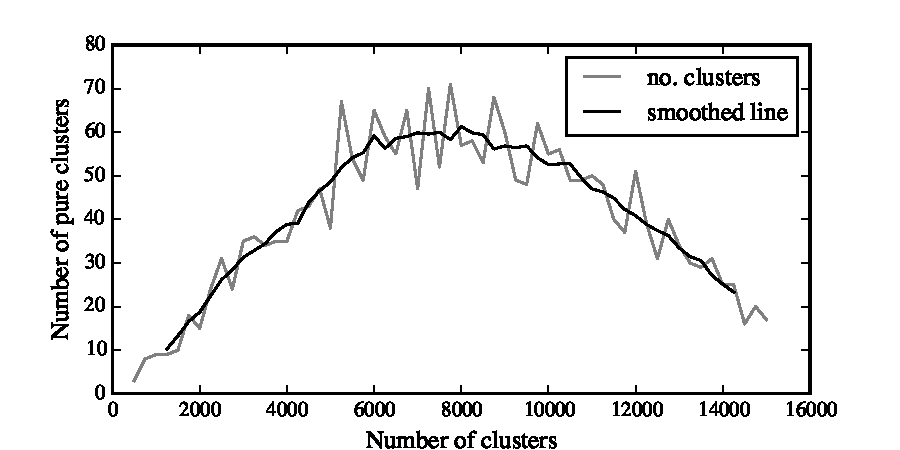
\includegraphics[width=0.9\textwidth]{pure-clusters.pdf}
\caption{}
\label{fig:k-vs-pureclusters}
\end{figure}


\begin{figure}[h]
\centering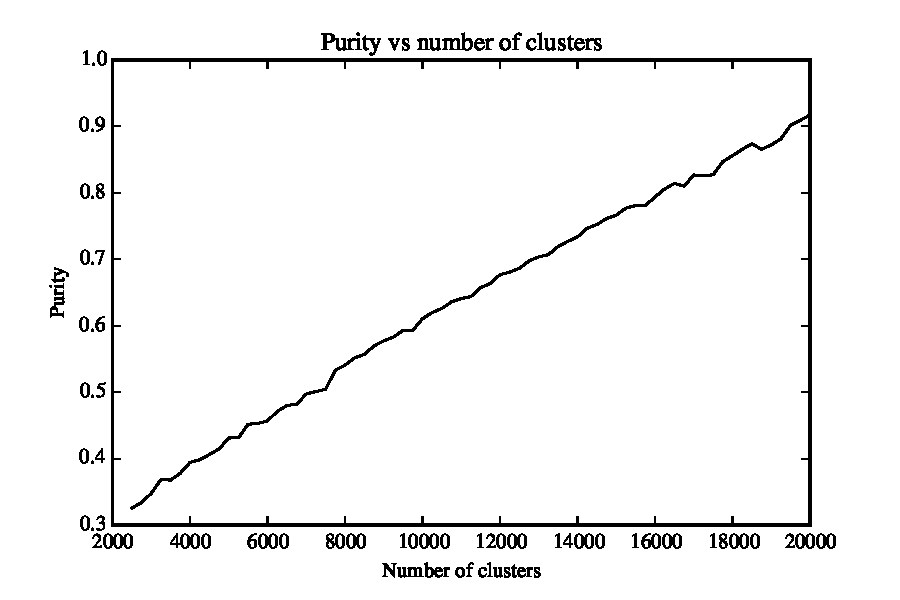
\includegraphics[width=0.9\textwidth]{purity.pdf}
\caption{}
\label{fig:k-vs-purity}
\end{figure}


\subsection{Building Hierarchy} \label{sec:hierarchy}


Once 

AMS Mathematics Subject Classification (2010) \cite{ams2010msc}
Excluded all subcategories those code end with '99': they are 
usually 'Miscellaneous topics' or 'None of the above, but in this section'. 
top level categories 'General', 'History and biography', and 'Mathematics education'
were also excluded. 
Additionally we exclude the following: 

\begin{itemize}
\item Quantum theory $\to$ Axiomatics, foundations, philosophy
\item Quantum theory $\to$ Applications to specific physical systems
\item Quantum theory $\to$ Groups and algebras in quantum theory
\item Partial differential equations $\to$ Equations of mathematical physics and other areas of application
\item Statistics $\to$ Sufficiency and information
\item Functional analysis $\to$ Other (nonclassical) types of functional analysis
\item Functional analysis $\to$ Miscellaneous applications of functional analysis
\end{itemize}

So these categories do not interfere with PACS. 


APS Physics and Astronomy Classification Scheme (2010) \cite{aps2010pacs}

We remove the ``GENERAL'' top-level category. 
In PACS there are 3 levels of categories, but we merge all 3-rd level categories into 
2nd level.

ACM Classification Scheme \cite{rous2012acm} available as a SKOS \cite{miles2005skos} ontology 
at their website \cite{amc2012ccs}. The SKOS ontology graph was processed with RDFLib \cite{rdflib}

We keep the following top level categories:
``Hardware'', ``Computer systems organization'', ``Networks'', 
``Software and its engineering'', ``Theory of computation'', 
``Information systems'', ``Security and privacy'',
``Human-centered computing'', ``Computing methodologies''.

After obtaining the data and parsing, all categories, the hierarchies 
are merged into one and then we try to match the found namespaces 
with second-level category in the hierarchy. 

This is done by keywords matching: we extract all words from the 
category (this includes top level category name, subcategory name
and all sub-sub categories concatenated). From the cluster 
we also extract the category information.
Then we try to do keyword matching using cosine similarity 
between the cluster and each category. The cluster is assigned 
to the category with the best cosine. 

If the cosine score is low (below $0.2$) or there is only one 
keyword matched, then the cluster is assigned to the ``OTHERS'' 
category.


\subsection{Java Language Processing} \label{sec:jlp}

The same set of techniques can be applied to source code.
(todo: why!)
If a language 
is statically typed, like Java or Pascal, usually it is possible to know the
type of a variable from its declaration. Therefore we can see 
variables as identifiers and types as "definitions" (TODO: clearly state 
the difference between types and definitions).

To extract this information from some source code repository each file source
file can be processed to obtain its Abstract Syntax Tree, and then 
declaration information can be extracted from it. 


In this word we process Java source code using JavaParser \cite{javaparser} - 
a library for parsing java source code. Java was chosen because the variable 
types always have to be declared, unlike other languages where the type 
can be inferred by compilers. 

The following declarations are processed: fields of a class, method and 
constructor parameters, inner variable declarations inside 
methods and constructors. It processes both usual classes and inner classes. 

\textbf{Add example and the results}


In the experiments we process Apache Mahout source code \cite{mahout}. 

Describe the dataset
